\documentclass[11pt]{article}

\usepackage[T1]{fontenc}
\usepackage{mathpazo}
\usepackage[utf8]{inputenc}
\usepackage[english]{babel}
\usepackage[margin=1in]{geometry}
\usepackage[protrusion=true,expansion=false]{microtype}
\usepackage{setspace}
\usepackage{amsmath, amssymb}
\usepackage{graphicx}
\usepackage{float}
\usepackage{subcaption}
\usepackage{booktabs}
\usepackage{array}
\usepackage{enumitem}
\usepackage{xcolor}
\usepackage{xurl}
\usepackage[hidelinks]{hyperref}
\usepackage[autostyle, english = american]{csquotes}
\usepackage[labelfont=bf, font=small]{caption}
\usepackage{titlesec}
\usepackage{fancyhdr}

\MakeOuterQuote{"}
\setstretch{1.15}
\setlength{\parindent}{1.5em}
\setlength{\parskip}{0.35em}
\setlist[itemize]{topsep=0.4em,itemsep=0.25em,leftmargin=1.8em}

\definecolor{sectionblue}{RGB}{34,67,120}
\titleformat{\section}{\large\bfseries\color{sectionblue}}{\thesection.}{0.6em}{}
\titleformat{\subsection}{\normalsize\bfseries}{\thesubsection.}{0.6em}{}
\titleformat{\subsubsection}{\normalsize\itshape}{\thesubsubsection.}{0.6em}{}

\setlength{\headheight}{14.5pt}
\pagestyle{fancy}
\fancyhf{}
\lhead{Twitch Dataset Report}
\rhead{\thepage}
\renewcommand{\headrulewidth}{0.4pt}

\captionsetup{justification=raggedright, singlelinecheck=false}

\newcommand{\reporttitle}{StatCrunch Competition: Twitch Dataset}
\newcommand{\reportauthor}{Matthew Carson\\University of California, Los Angeles}
\newcommand{\reportdate}{April 30, 2024}

\begin{document}

\begin{titlepage}
    \centering
    \vspace*{2.5cm}
    {\LARGE \bfseries \reporttitle\par}
    \vspace{1.5cm}
    {\large Final Report\par}
    \vspace{2cm}
    {\large \reportauthor\par}
    \vfill
    {\large \reportdate\par}
\end{titlepage}

\pagenumbering{roman}

\section*{Executive Overview}
This report analyzes the top 900 Twitch accounts in the StatCrunch competition dataset. The main goal is descriptive rather than inferential: to summarize patterns in streaming, viewership, follower growth, and partnered status among these accounts. Across the analyses, several findings are counterintuitive. Accounts that stream more hours tend to have fewer average viewers, and greater streaming time is only weakly related to follower counts. Mature accounts also tend to have fewer followers, although differences in watch time explain only a modest share of that gap. Finally, follower count is the strongest single predictor of partnered status.

\tableofcontents
\listoftables
\listoffigures
\newpage

\pagenumbering{arabic}

\section{Introduction}
This paper examines relationships within a dataset of the top 900 Twitch accounts. The analyses focus on three broad questions: how streaming time relates to audience outcomes, whether mature accounts differ from non-mature accounts in follower counts, and which variable best predicts partnered status.

The document is organized as follows. Section 2 describes the data and measurement decisions. Section 3 presents descriptive results and correlations. Sections 4 through 6 present the regression analyses. Section 7 concludes, and the appendix collects supporting figures and tables.

\section{Data, Scope, and Measurement}

\subsection{Scope of the Analysis}
Because these data were not randomly sampled, inferential statistics are not appropriate. Confidence intervals and hypothesis tests would invite population claims that the data cannot support. The analyses therefore remain descriptive and model-based within the observed population of top Twitch accounts.

\subsection{Variable Construction}
Before presenting the summary statistics, two high-magnitude variables were rescaled to improve interpretability:

\begin{equation}
\text{Mean weekly watch hours} = \frac{\text{Watch time (mins)}}{60 \times 52}
\end{equation}

\begin{equation}
\text{Mean weekly stream hours} = \frac{\text{Stream time (mins)}}{60 \times 52}
\end{equation}

Additional derived variables were also calculated.\footnote{Entire dataset available at \href{https://www.statcrunch.com/app/index.html?dataid=4597814&token=OTI3Z8\%2F0N6hSC1KVw9hTXmyjHLnuZvqCMyuxkgn1QRYPhIQfDVLUFClF3Y41ShOi4C\%2BMKL5\%2FHgpBTXKukjWOPGD4pN\%2FCkiobeyKouIjPB7LoPvHOTDN7wUNtPZQd2\%2BNjOwAtSMQl9aKQrbthjCSuuSihsliiTo0MvakPDYN0lwiE8N11ITBSTS9QJH9QgHEmO4ahoV6IkASuVdKosV\%2FJSQ\%3D\%3D}{StatCrunch}.}

\begin{itemize}
    \item \texttt{Followers Prev Yr} = \texttt{Followers} - \texttt{Followers gained}
    \item \texttt{Followers gained percent} = \texttt{Followers gained} / \texttt{Followers Prev Yr}
\end{itemize}

\section{Descriptive Results}

\subsection{Summary Statistics}
The distributions are heavily right-skewed, so medians are more informative than means for most variables.

\begin{table}[H]
  \centering
  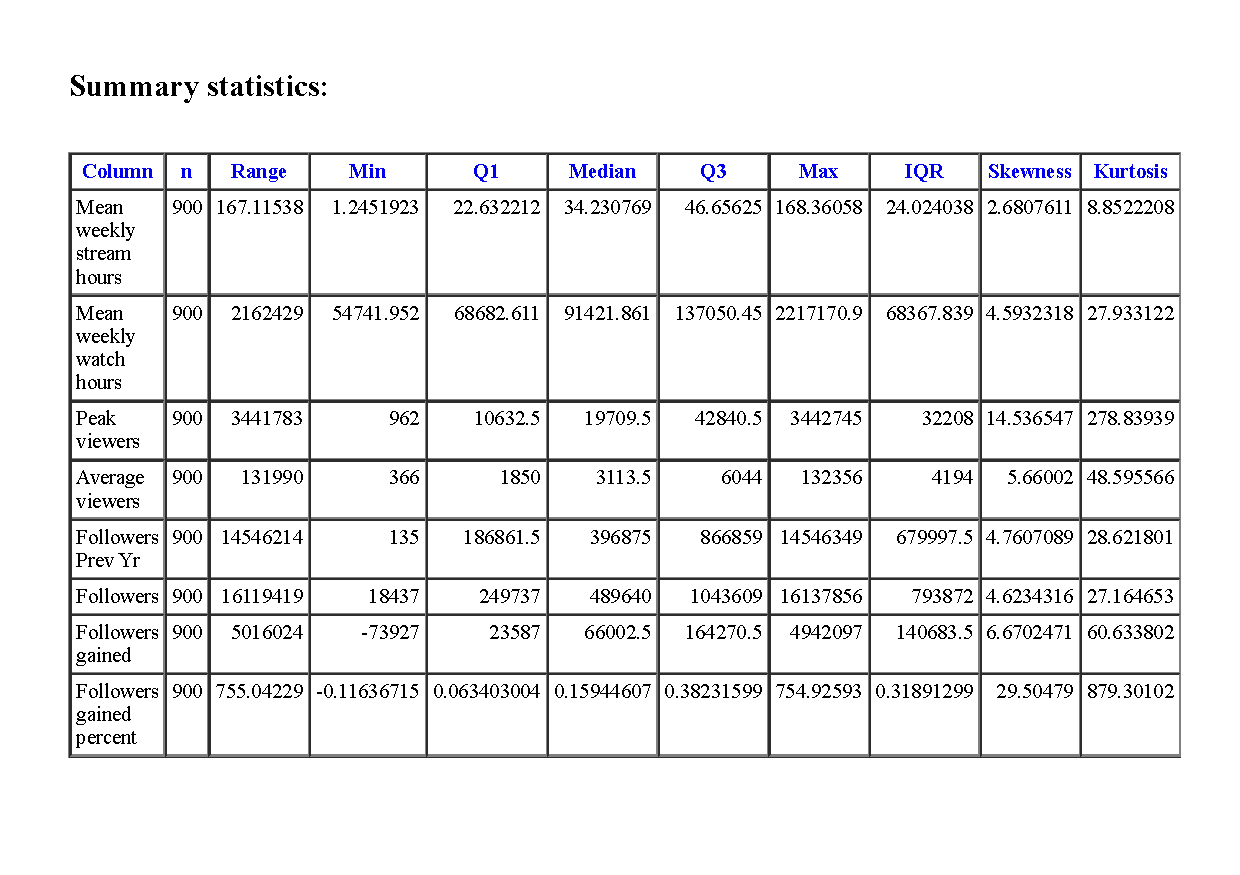
\includegraphics[width=0.84\linewidth]{../StatCrunch_Results/table}
  \caption{Summary statistics for the Twitch dataset.}
  \label{table:summary_stats}
\end{table}

All distributions are heavily right-skewed, with skewness values at or above 2.6. For that reason, medians are emphasized throughout this report. The median account streams about 34.23 hours per week and is watched roughly 91{,}422 hours per week. Median follower growth is also substantial: the typical account gained about 66{,}003 followers over the period, a median increase of roughly 16 percent. The underlying skewness also makes compact visual summaries difficult to read cleanly, as shown in Figure \ref{fig:histogram_matrix}.

\subsection{Correlation Patterns}
Spearman's rank correlations were used to assess relationships among the numeric variables because the observed relationships are generally non-linear.

\begin{figure}[H]
  \centering
  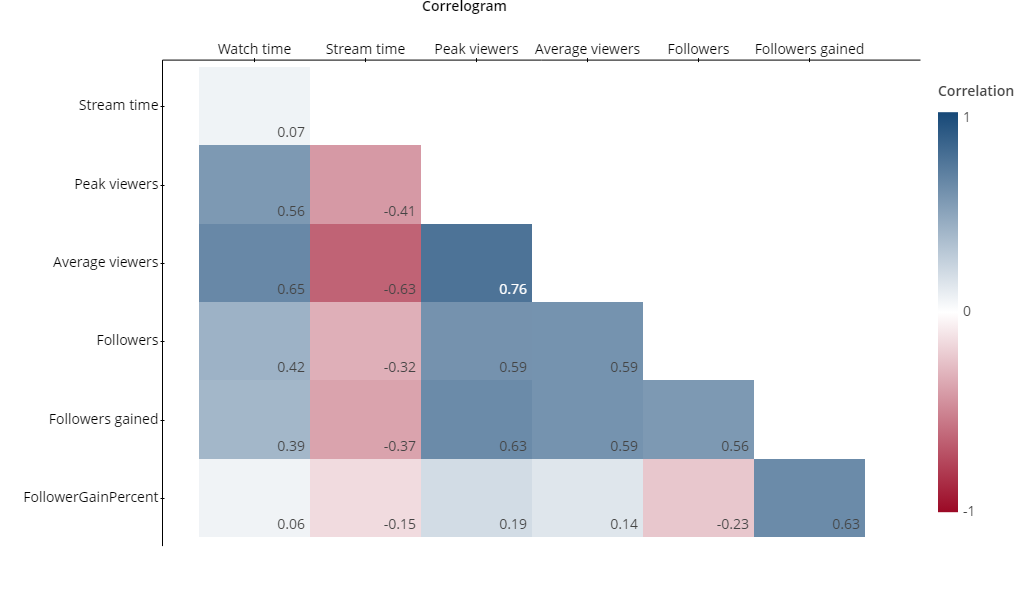
\includegraphics[width=\linewidth]{../StatCrunch_Results/spearman_correlogram}
  \caption{Spearman correlation matrix for the numeric variables.}
  \label{fig:spearman_correlogram}
\end{figure}

Several of the observed relationships are striking. Mean weekly stream hours has a moderately strong negative association with average viewers ($\rho = -0.63$), which runs against the intuition that streaming more should expand an account's audience. At the same time, stream time is nearly unrelated to watch time ($\rho = 0.07$). These patterns suggest that greater streaming volume alone does not translate into larger audiences.

The same pattern appears when follower growth is compared across stream-time deciles.

\begin{table}[H]
  \centering
  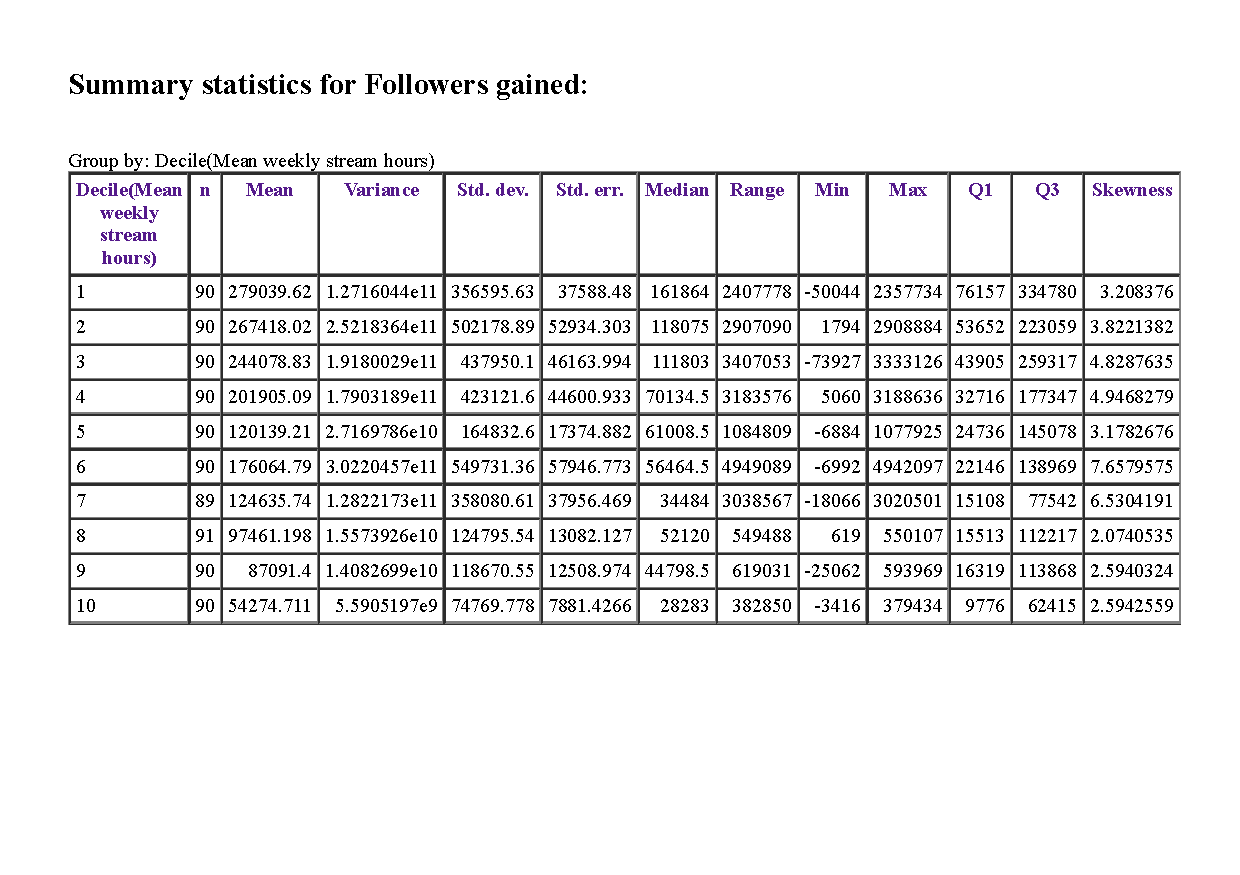
\includegraphics[width=0.90\linewidth]{../StatCrunch_Results/followers_gained_stream_deciles/table}
  \caption{Followers gained across deciles of stream time. The first decile contains the accounts with the fewest streaming hours.}
  \label{table:followers_gained_stream_decile_table}
\end{table}

\begin{figure}[H]
  \centering
  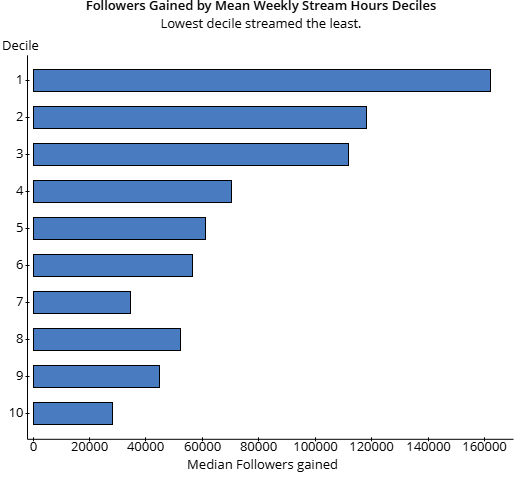
\includegraphics[width=0.64\linewidth]{../StatCrunch_Results/followers_gained_stream_deciles/barplot}
  \caption{Followers gained across deciles of stream time. The first decile contains the accounts with the fewest streaming hours.}
  \label{fig:followers_gained_stream_deciles}
\end{figure}

Accounts in the highest stream-time decile gained far fewer followers than accounts in the lowest decile. Taken together, the descriptive evidence suggests that simply streaming more often is not an effective stand-alone strategy for audience growth.

\section{Simple Linear Regression Analyses}
Because several relationships were clearly non-linear, transformations were used where necessary to obtain more interpretable linear fits.

\subsection{Stream Hours and Average Viewers}
A first question is whether accounts that stream more hours also attract more viewers. The raw relationship is strongly non-linear, so \texttt{Average viewers} was transformed using its reciprocal.

\subsubsection{Model}
\begin{equation}
\frac{1}{\text{Average viewers}_{i}} = \beta_{0} + \beta_{1}(\text{Mean weekly stream hours}_{i})
\end{equation}

where $i$ indexes Twitch accounts.

\subsubsection{Results}
\begin{table}[H]
  \centering
  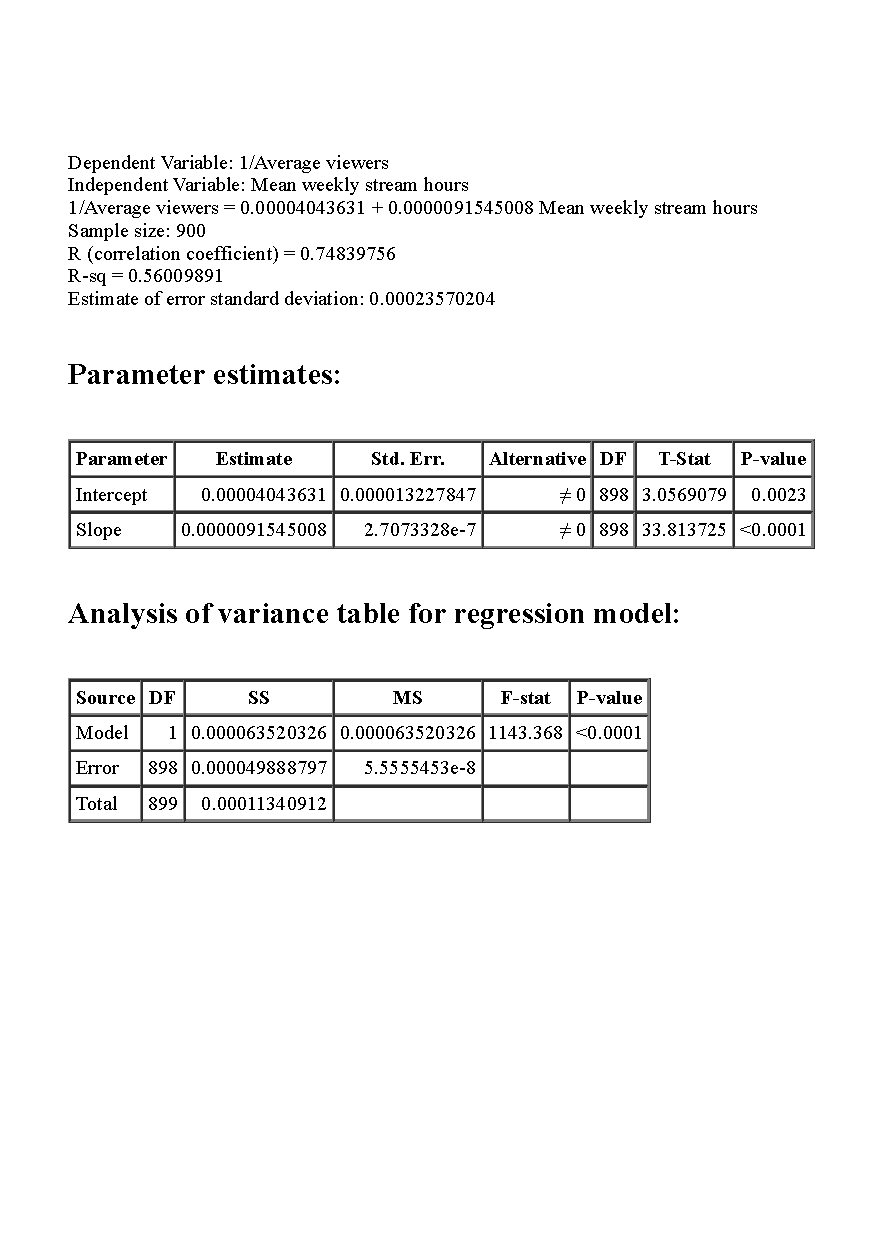
\includegraphics[scale=0.75]{../StatCrunch_Results/reciprocal/regression_table}
  \caption{Simple linear regression of reciprocal average viewers on mean weekly stream hours.}
  \label{table:reciprocal_regression_table}
\end{table}

The model explains a moderate share of the variation in the transformed outcome ($R^2 = 0.56$). Because the dependent variable is the reciprocal of average viewers, the coefficient signs reverse the intuitive direction on the original scale. After back-transformation, the substantive pattern is clear: more weekly stream hours are associated with fewer average viewers.

\begin{equation}
\frac{1}{\text{Average viewers}_i} = 4.043631\times10^{-5} + 9.1545008\times10^{-6}(\text{Mean weekly stream hours}_i)
\label{eq:reciprocal_model_w_coef}
\end{equation}

\begin{figure}[H]
  \centering
  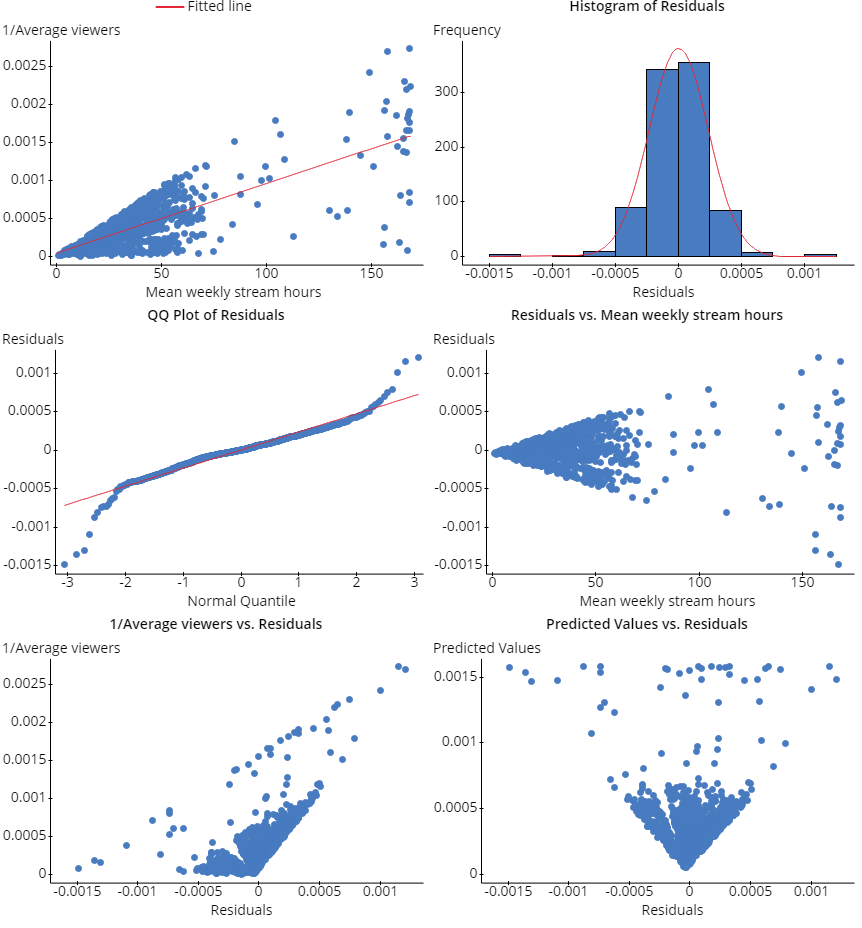
\includegraphics[scale=0.5]{../StatCrunch_Results/reciprocal/stream_time_reciprocal_avg_viewers_plots}
  \caption{Diagnostic plots for the reciprocal-average-viewers model.}
  \label{fig:stream_time_reciprocal_avg_viewers}
\end{figure}

To restore interpretability, the fitted relationship can be expressed on the original viewer scale:

\begin{equation}
\text{Average viewers}_i = \frac{1}{4.043631\times10^{-5} + 9.1545008\times10^{-6}(\text{Mean weekly stream hours}_i)}
\label{eq:back_transformed_reciprocal_eq}
\end{equation}

\begin{figure}[H]
  \centering
  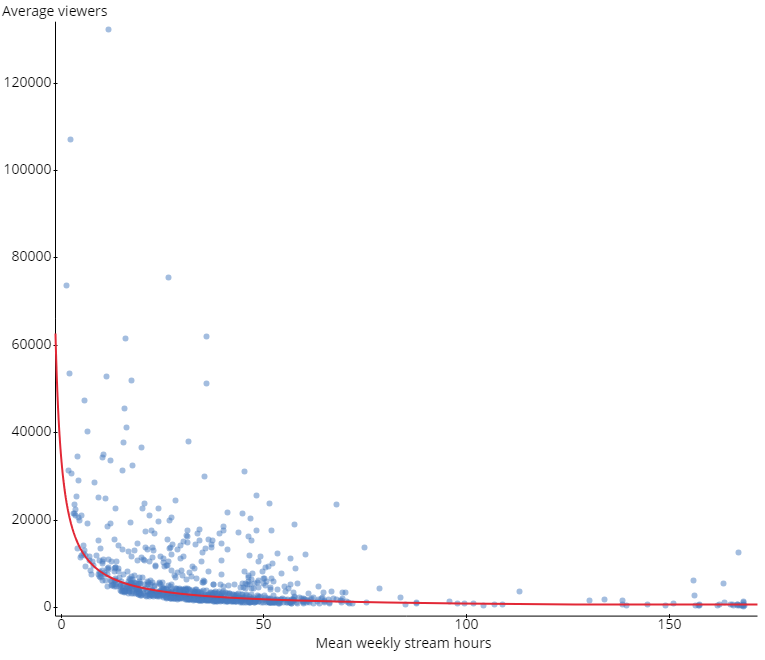
\includegraphics[width=0.80\linewidth]{../StatCrunch_Results/reciprocal/scatter_plot_reverse_transformed}
  \caption{Back-transformed fitted values for average viewers as a function of mean weekly stream hours.}
  \label{fig:transformed_reciprocal_scatter}
\end{figure}

At the sample median of 34.23 weekly stream hours, the model predicts about 2{,}826 average viewers. Ten fewer hours of weekly streaming raises the predicted value to about 3{,}813, a difference of roughly 987 viewers.

\subsection{Stream Hours and Followers}
A second question is whether more streaming time is associated with more followers. The raw relationship again appears non-linear, so \texttt{Followers} was log-transformed.

\subsubsection{Model}
\begin{equation}
\ln(\text{Followers}_{i}) = \beta_{0} + \beta_{1}(\text{Mean weekly stream hours}_{i})
\label{eq:ln_followers_stream}
\end{equation}

\subsubsection{Results}
\begin{table}[H]
\centering
  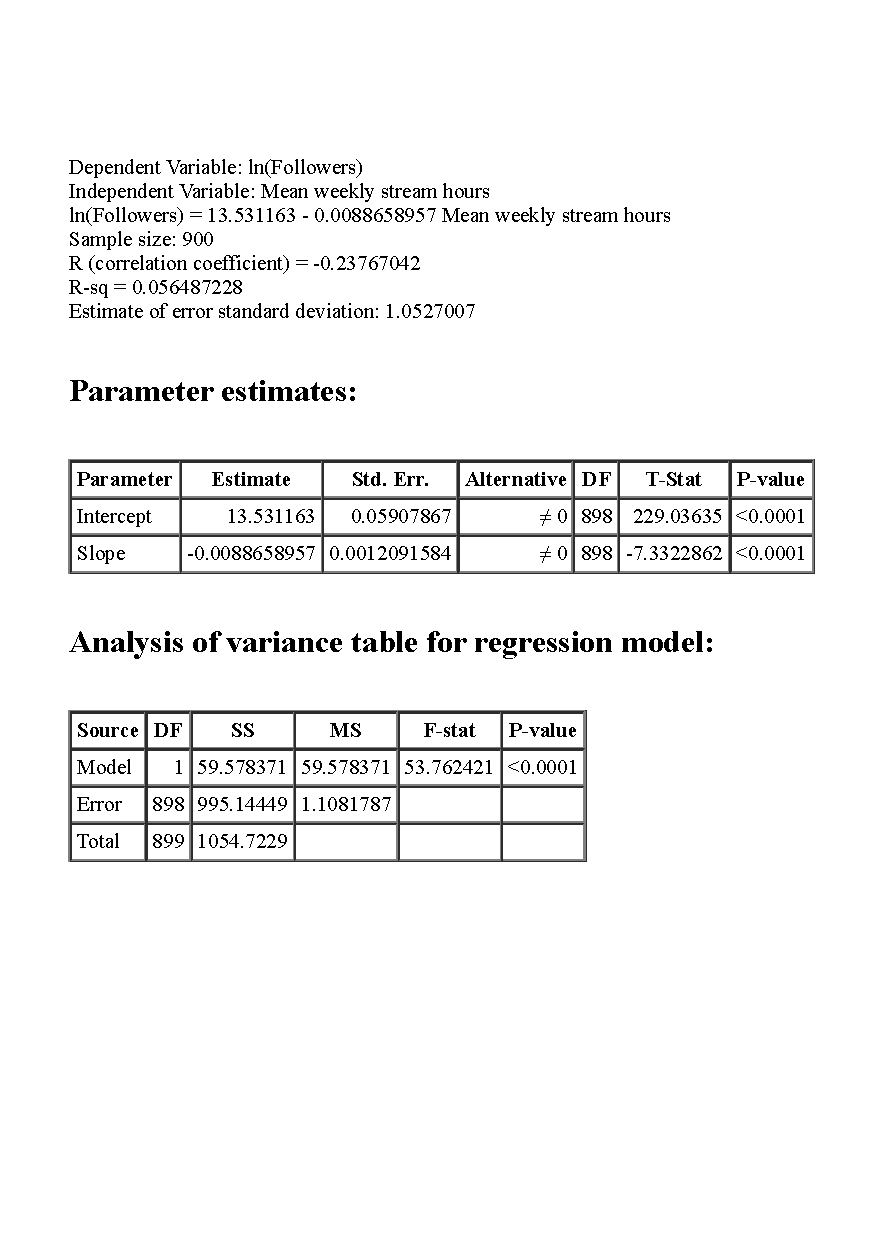
\includegraphics[height=0.5\textheight]{../StatCrunch_Results/ln_followers_stream/table}
  \caption{Simple linear regression of logged followers on mean weekly stream hours.}
  \label{tab:ln_followers_stream}
\end{table}

\begin{figure}[H]
\centering
    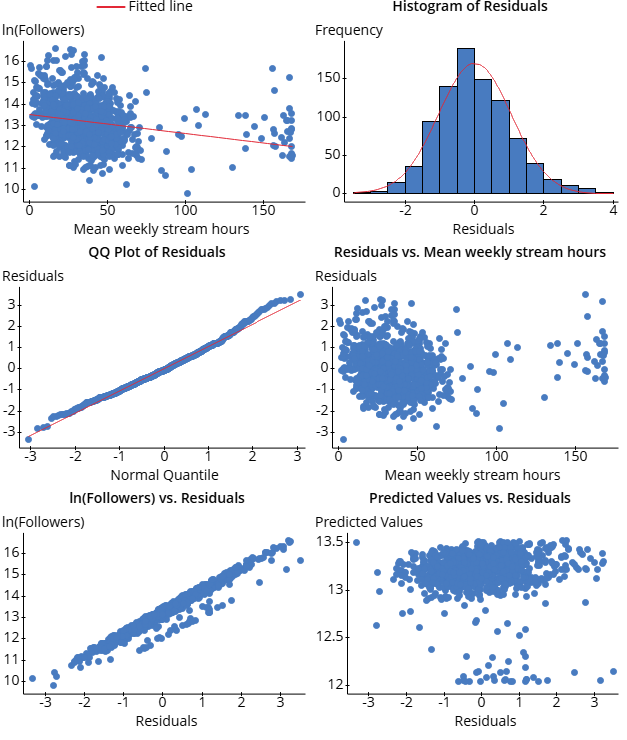
\includegraphics[height=0.68\textheight]{../StatCrunch_Results/ln_followers_stream/plot}
    \caption{Diagnostic plots for the model of logged followers on mean weekly stream hours.}
    \label{fig:ln_followers_stream_plot}
\end{figure}

\begin{figure}[H]
\centering
    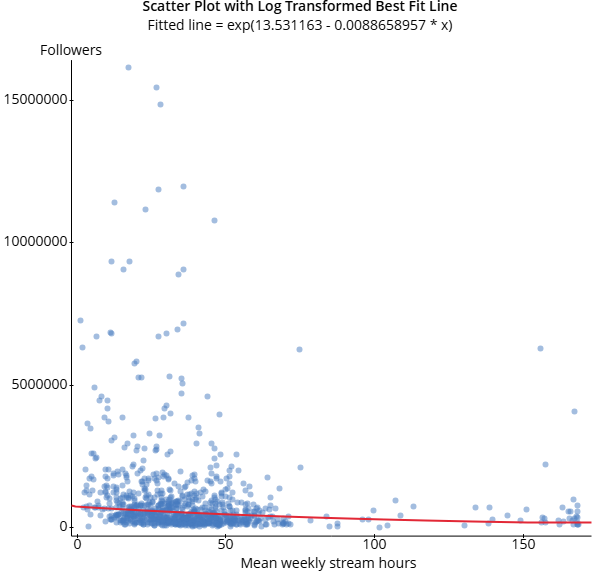
\includegraphics[scale=0.65]{../StatCrunch_Results/ln_followers_stream/scatter_small}
    \caption{Logged followers regressed on mean weekly stream hours.}
    \label{fig:ln_followers_stream_scatter}
\end{figure}

The fitted relationship is weakly negative, with $R^2 = 0.056$. Exponentiating the coefficient on mean weekly stream hours implies that each additional weekly stream hour is associated with about 0.88 percent fewer followers. This is a weak relationship, but it points in the same direction as the earlier descriptive results.

\section{Multiple Linear Regression}

\subsection{Mature Classification and Followers}
This section asks whether differences in watch time help account for the follower gap between mature and non-mature accounts.

\subsubsection{Difference in Means}
Because \texttt{Followers} is strongly skewed, the analysis begins with the log of followers. The mean difference in logged followers between mature and non-mature accounts is $-0.13351611$. Exponentiating this value yields $0.875$, which implies that mature accounts have about 12.5 percent fewer followers on average.

\begin{equation}
\begin{aligned}
\mu_{1} &= \text{Mean of } \ln(\text{Followers}) \text{ for mature accounts} \\
\mu_{2} &= \text{Mean of } \ln(\text{Followers}) \text{ for non-mature accounts} \\
\mu_{1} - \mu_{2} &= -0.13351611 \\
\exp(-0.13351611) &= 0.875
\end{aligned}
\label{eq:log_means_followers_mature}
\end{equation}

\subsubsection{Model}
\begin{equation}
\ln(\text{Followers}_{i}) = \beta_{0} + \beta_{1}(\text{Mature}_{i}) + \beta_{2}\ln(\text{Mean weekly watch hours}_{i})
\label{eq:multi_linear_model}
\end{equation}

\subsubsection{Results}
\begin{table}[H]
  \centering
  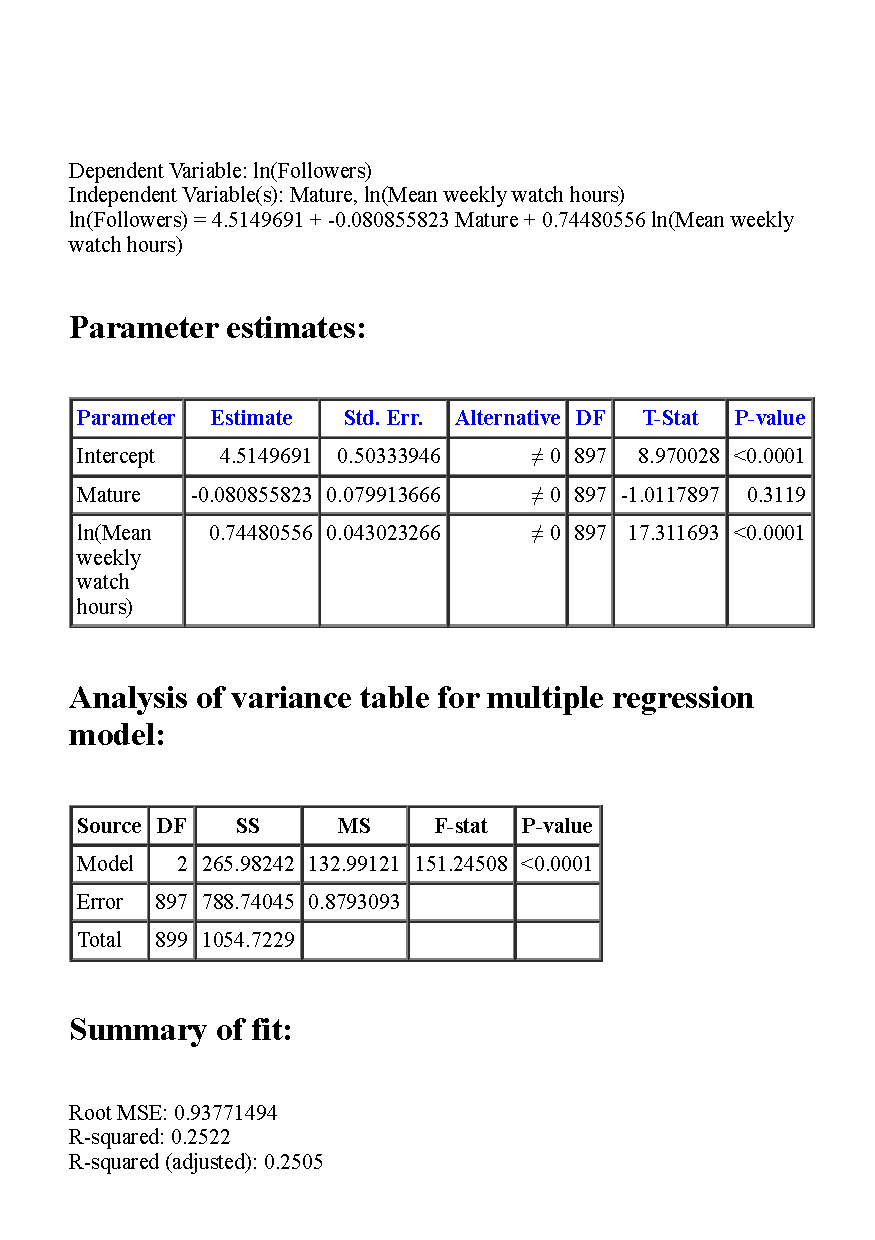
\includegraphics[scale = 0.7]{../StatCrunch_Results/followers_mature_watch_hrs/multi_regression_table}
  \caption{Multiple linear regression of logged followers on mature classification and logged weekly watch hours.}
  \label{tab:multi_regression_tab}
\end{table}

\begin{figure}[H]
    \centering
    \begin{subfigure}{0.47\textwidth}
        \centering
        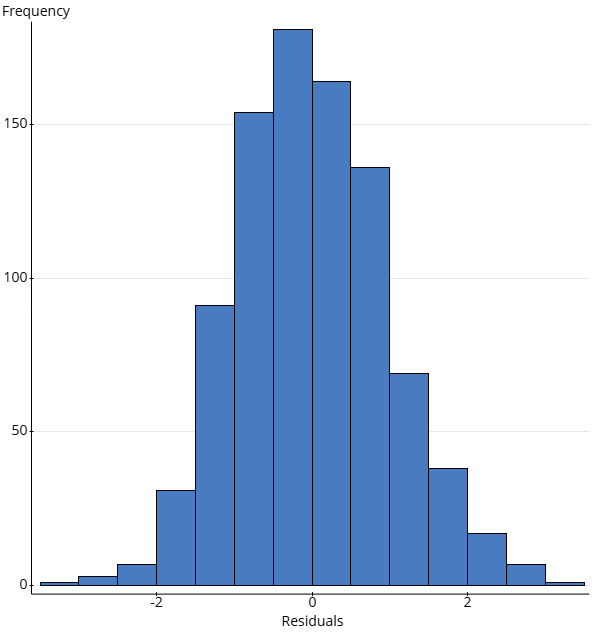
\includegraphics[width=\textwidth]{../StatCrunch_Results/followers_mature_watch_hrs/residual_histogram}
        \caption{Residual histogram}
        \label{fig:plot1}
    \end{subfigure}
    \hfill
    \begin{subfigure}{0.47\textwidth}
        \centering
        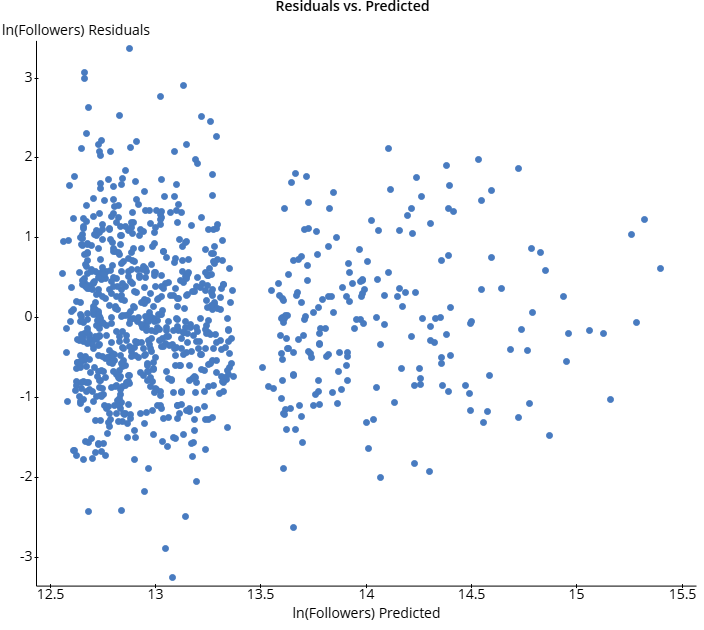
\includegraphics[width=\textwidth]{../StatCrunch_Results/followers_mature_watch_hrs/residual_plot}
        \caption{Residuals versus fitted values}
        \label{fig:plot2}
    \end{subfigure}
    \caption{Diagnostics for the multiple linear regression model.}
    \label{fig:both_plots}
\end{figure}

The model has modest explanatory power ($R^2 = 0.25$). The coefficient on \texttt{Mature} is $-0.080855823$, which becomes $0.9223$ after exponentiation. Holding logged weekly watch hours constant, mature accounts therefore have about 7.7 percent fewer followers than non-mature accounts. The drop from 12.5 percent in the raw comparison to 7.7 percent in the adjusted model indicates that differences in watch time explain some, but not most, of the follower gap.

\section{Logistic Regression}

\subsection{Predicting Partnered Status}
The final question is which variable best predicts whether a Twitch account is partnered. Separate one-predictor logistic models were fit and compared using Akaike's information criterion (AIC).

\subsubsection{Model Comparison}
\begin{table}[H]
\centering
\caption{AIC values for one-predictor models of partnered status. Lower values indicate better fit among models with comparable complexity.}
\label{tab:aic_single}
\begin{tabular}{@{}lr@{}}
\toprule
Predictor & AIC \\
\midrule
\texttt{Followers} & 237.57 \\
\texttt{Peak viewers} & 245.79 \\
\texttt{Average viewers} & 246.42 \\
\texttt{Mature} & 246.22 \\
\texttt{Mean weekly watch hours} & 245.77 \\
\texttt{Mean weekly stream hours} & 246.36 \\
\bottomrule
\end{tabular}
\end{table}

\begin{table}[H]
\centering
\caption{AIC values for models that add one additional predictor to \texttt{Followers}.}
\label{tab:aic_multi}
\begin{tabular}{@{}lr@{}}
\toprule
Predictors & AIC \\
\midrule
\texttt{Followers + Peak viewers} & 238.80 \\
\texttt{Followers + Average viewers} & 237.67 \\
\texttt{Followers + Mature} & 239.07 \\
\texttt{Followers + Mean weekly watch hours} & 239.07 \\
\texttt{Followers + Mean weekly stream hours} & 238.32 \\
\bottomrule
\end{tabular}
\end{table}

\texttt{Followers} produces the lowest AIC among the one-predictor models, and adding any one additional variable fails to improve fit. The final logistic model therefore uses only follower count.

\subsubsection{Model}
Followers was rescaled by dividing by 100{,}000 so that the coefficient would be easier to interpret.

\begin{equation}
\log\left(\frac{p_i}{1-p_i}\right) = \beta_0 + \beta_1(\text{Followers}/100{,}000)_i
\end{equation}

where $p_i$ is the probability that account $i$ is partnered.

\subsubsection{Results}
\begin{table}[H]
  \centering
  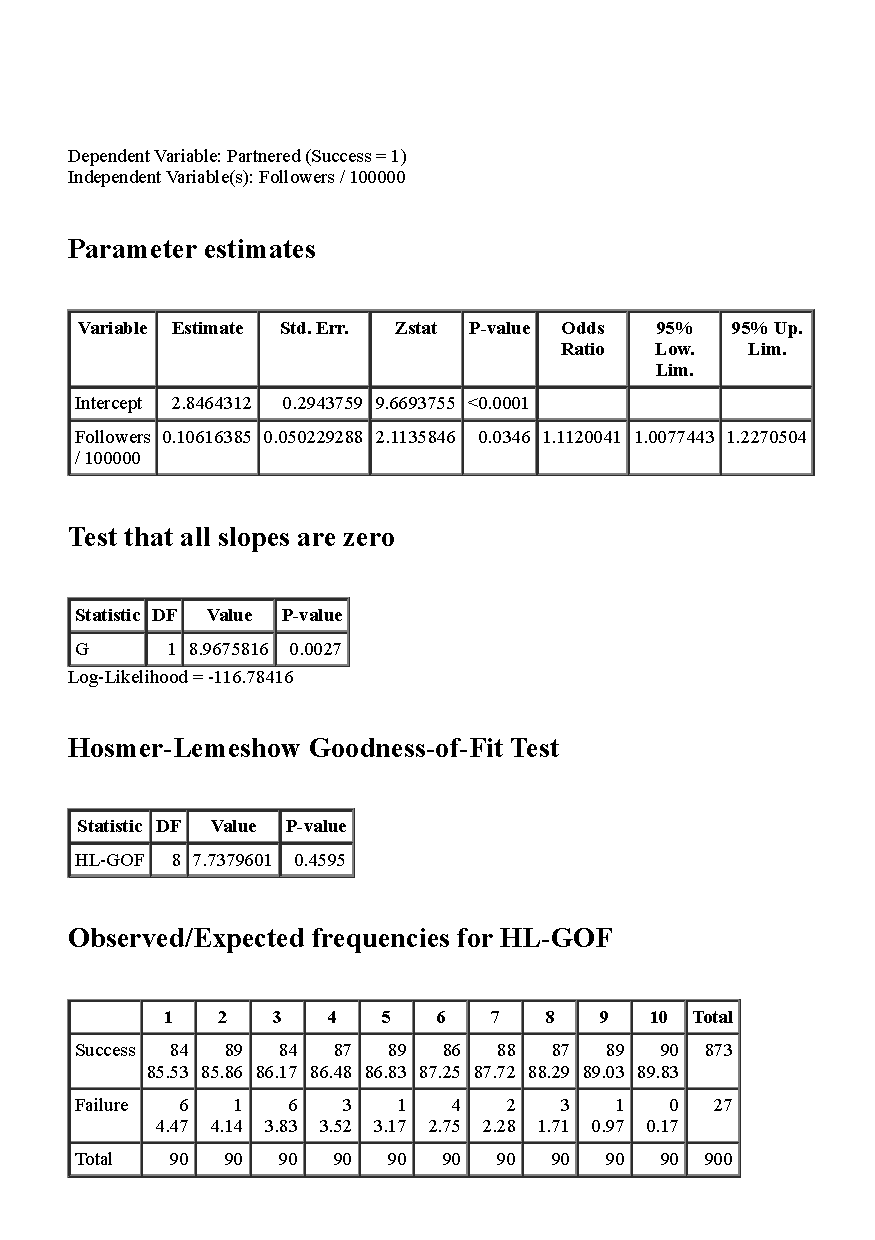
\includegraphics[scale=1]{../StatCrunch_Results/logit_partnered_followers/table}
  \caption{Logistic regression of partnered status on follower count.}
  \label{tab:logistic_table}
\end{table}

The estimated coefficient on \texttt{Followers / 100,000} is positive. Exponentiating that coefficient yields an odds ratio of 1.112, which means that each additional 100{,}000 followers is associated with an 11.2 percent increase in the odds of partnered status.

To make the fitted probabilities easier to visualize, the binary partnered indicator was jittered slightly before plotting.

\begin{equation}
\text{PartneredNoise} = 
\begin{cases}
    \text{Partnered} + |\text{Normal}| & \text{if } \text{Partnered} = 1 \\
    \text{Partnered} - |\text{Normal}| & \text{if } \text{Partnered} = 0
\end{cases}
\end{equation}

\begin{equation}
\hat{p}_{i} = \frac{e^{2.8464312 + 0.10616385(\text{Followers}/100{,}000)}}{1 + e^{2.8464312 + 0.10616385(\text{Followers}/100{,}000)}}
\end{equation}

\begin{figure}[H]
\centering
    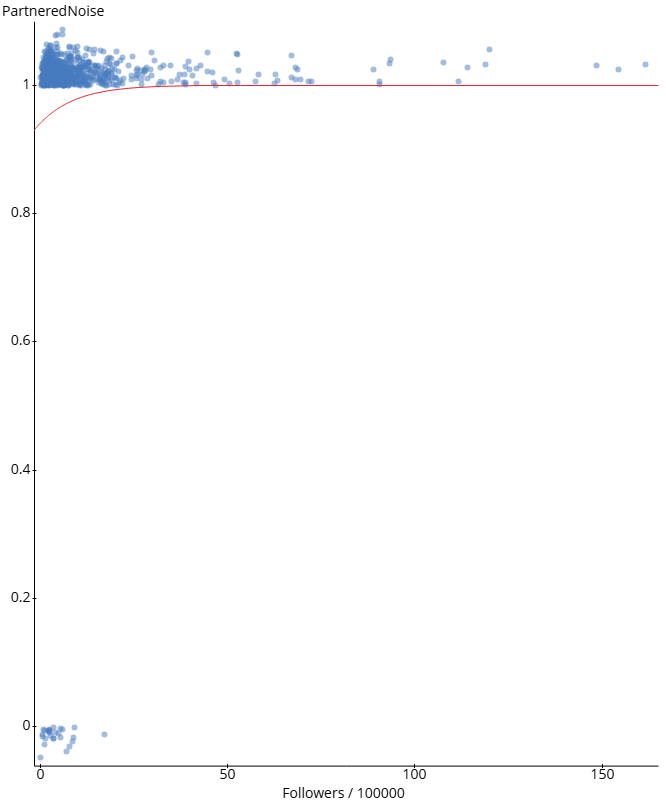
\includegraphics[width=0.75\linewidth]{../StatCrunch_Results/logit_partnered_followers/scatter_plot}
    \caption{Predicted probability of partnered status as a function of follower count.}
    \label{fig:logit_partnered_followers}
\end{figure}

The model appears reasonably calibrated overall, although it is more limited in predicting non-partnered status. That is likely due to the severe class imbalance in the dataset: 873 partnered accounts and only 27 non-partnered accounts.

\section{Conclusion}
Three conclusions stand out. First, more streaming time is not associated with better audience outcomes in this dataset; if anything, the relationship often runs in the opposite direction. Second, mature accounts have fewer followers than non-mature accounts, and differences in watch time explain only a modest part of that gap. Third, follower count is the strongest single predictor of partnered status.

These results should be interpreted descriptively. Because the dataset is not a random sample of Twitch users, the report does not support broader population inference. Even so, the observed patterns are clear and substantively interesting, especially where they contradict common intuitions about platform growth.

\appendix
\section{Appendix}

\subsection{Additional Figures}

\begin{figure}[H]
  \centering
  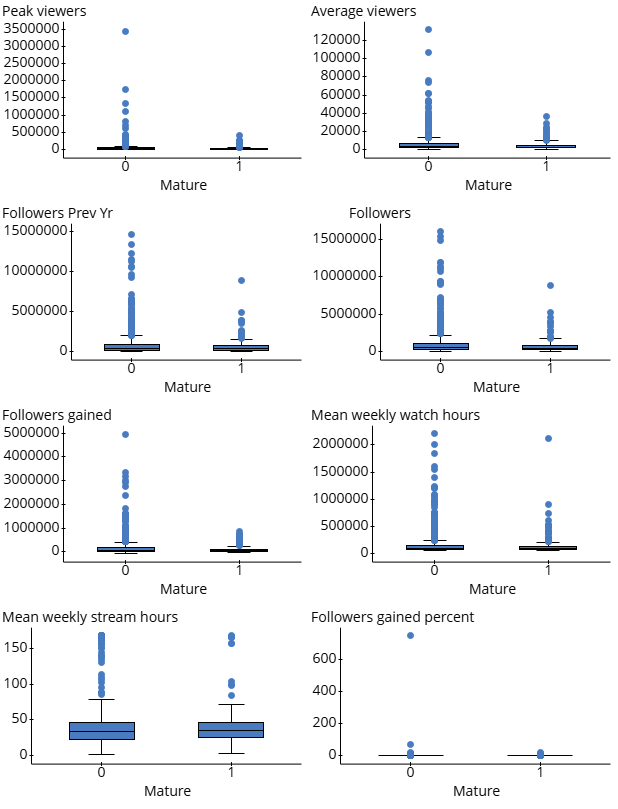
\includegraphics[width=0.8\linewidth]{../StatCrunch_Results/mature/box_plots}
  \caption{Box plots for Twitch accounts by mature classification.}
  \label{fig:box_plots_mature}
\end{figure}

\begin{figure}[H]
  \centering
  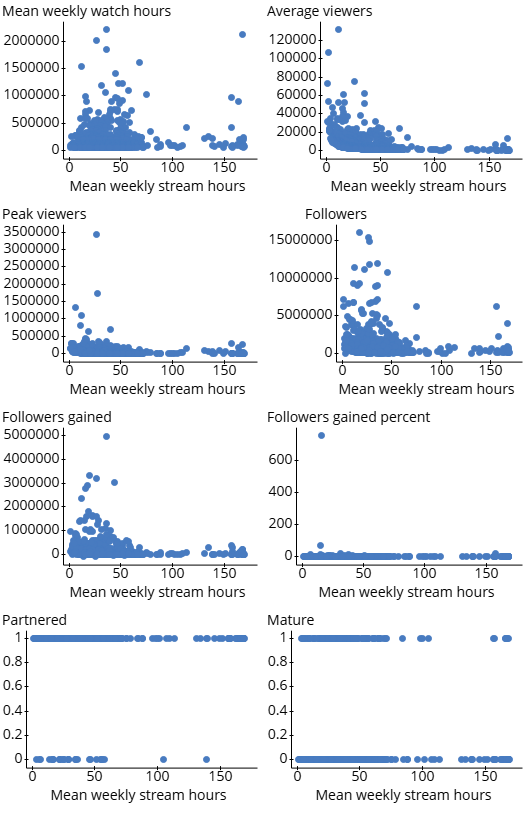
\includegraphics[width=0.795\linewidth]{../StatCrunch_Results/stream_scatter_plot_matrix.png}
  \caption{Relationships between mean weekly stream hours and other variables.}
  \label{fig:stream_scatter_matrix}
\end{figure}

\begin{figure}[H]
  \centering
  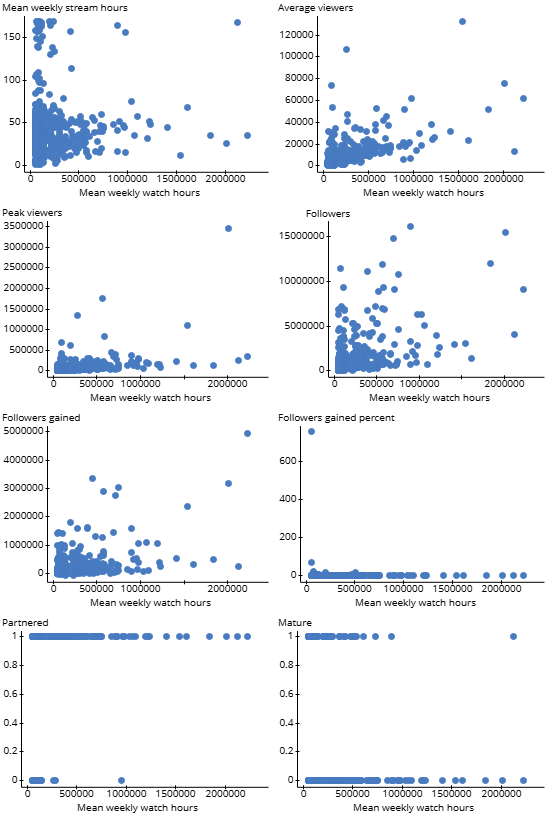
\includegraphics[width=0.8\linewidth]{../StatCrunch_Results/watch_scatter_plot_matrix.png}
  \caption{Relationships between mean weekly watch hours and other variables.}
  \label{fig:watch_scatter_matrix}
\end{figure}

\begin{figure}[H]
  \centering
  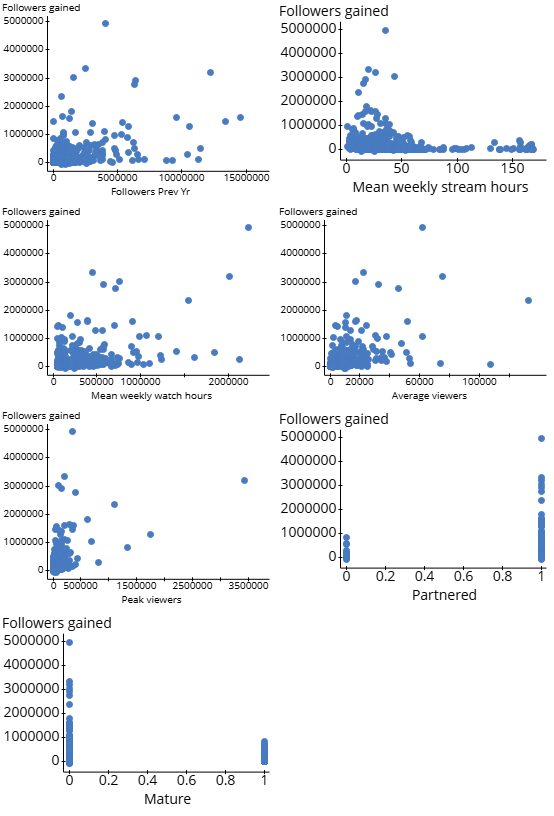
\includegraphics[width=0.8\linewidth]{../StatCrunch_Results/follow_gain_scatter_matrix}
  \caption{Relationships between followers gained and other variables.}
  \label{fig:follow_gain_scatter_matrix}
\end{figure}

\begin{figure}[H]
  \centering
  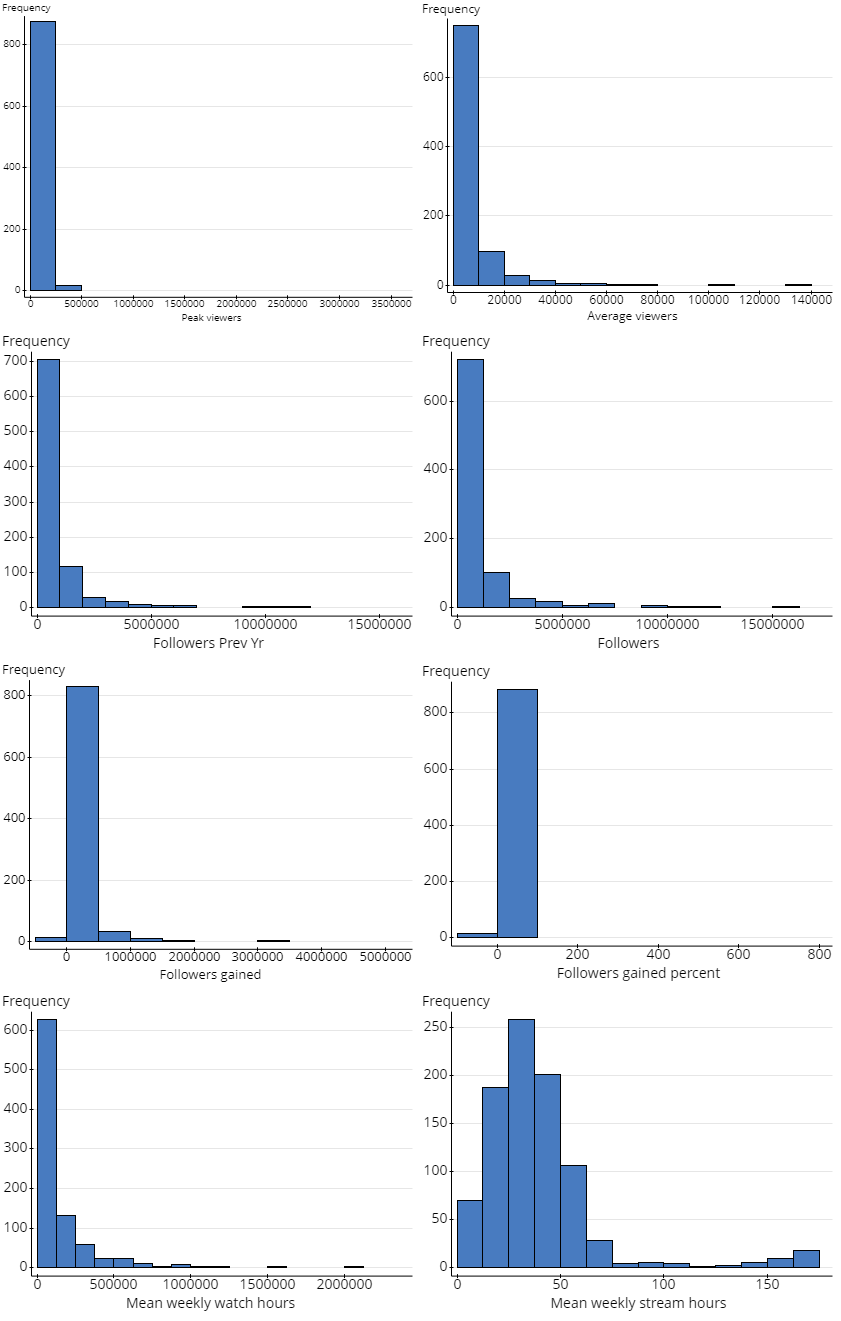
\includegraphics[width=0.8\linewidth]{../StatCrunch_Results/Histogram_Matrix.png}
  \caption{Histogram matrix showing strong skew across the variables.}
  \label{fig:histogram_matrix}
\end{figure}

\begin{table}[H]
  \centering
  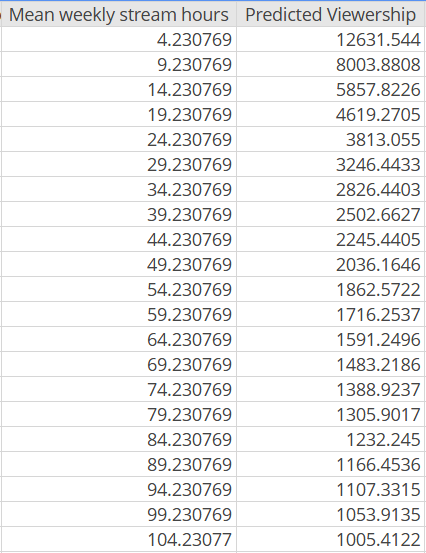
\includegraphics[scale=1]{../StatCrunch_Results/reciprocal/prediction_matrix}
  \caption{Predicted values from the back-transformed reciprocal model.}
  \label{tab:prediction_matrix}
\end{table}

\subsection{StatCrunch Dataset Link}
\noindent\url{https://www.statcrunch.com/app/index.html?dataid=4597814&token=OTI3Z8\%2F0N6hSC1KVw9hTXmyjHLnuZvqCMyuxkgn1QRYPhIQfDVLUFClF3Y41ShOi4C\%2BMKL5\%2FHgpBTXKukjWOPGD4pN\%2FCkiobeyKouIjPB7LoPvHOTDN7wUNtPZQd2\%2BNjOwAtSMQl9aKQrbthjCSuuSihsliiTo0MvakPDYN0lwiE8N11ITBSTS9QJH9QgHEmO4ahoV6IkASuVdKosV\%2FJSQ\%3D\%3D}

\end{document}
